\newpage
\subsection{Implementing invert}
\visHeader
\hypertarget{invertCard vis}{}

\begin{itemize}

\vspace{0.5cm}

\item[$\blacktriangleright$] You're no longer an SDM beginner, so model the simple control flow depicted in Fig.~\ref{fig:sdm_invertEmpty}. 

\vspace{0.5cm}

\begin{figure}[htbp]
\begin{center}
  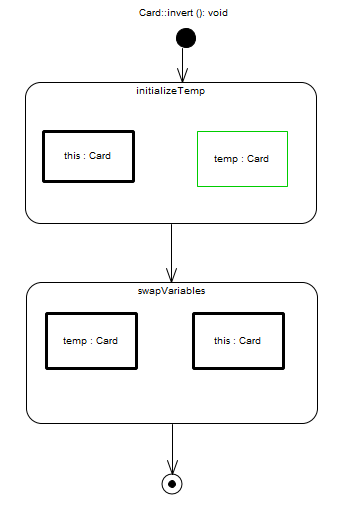
\includegraphics[width=0.6\textwidth]{ea_invertEmpty}
  \caption{Swap back and face of the card}  
  \label{fig:sdm_invertEmpty}
\end{center}
\end{figure}

\vspace{0.5cm}

\item[$\blacktriangleright$] This activity will need four assignment constraints - two in \texttt{initialize temp} to store the opposite values in
\texttt{temp}, and two in \texttt{swap variables} to set the new values. Create your first assignment constraint by going to the created \texttt{temp} card and
using the `\texttt{:=}' operator to set the \texttt{temp.back} value to \texttt{this.face} (Fig.~\ref{fig:sdm_invertAssignment}).

\begin{figure}[htbp]
\begin{center}
  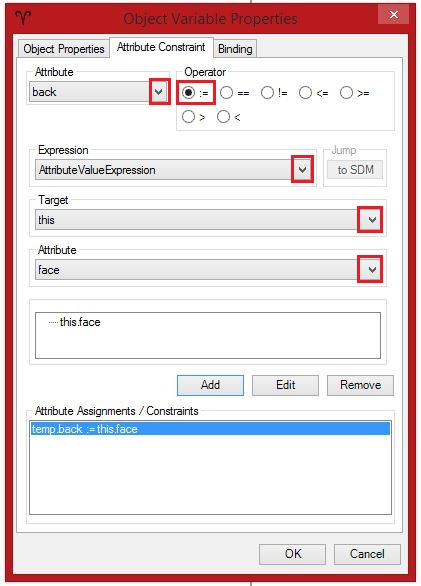
\includegraphics[width=0.7\textwidth]{ea_invertAttConstAssign}
  \caption{Swap back and face of the card}  
  \label{fig:sdm_invertAssignment}
\end{center}
\end{figure}

\clearpage

\vspace*{0.5cm}

\item[$\blacktriangleright$] Complete the SDM with the remaining constraints according to Fig~\ref{fig:sdm_invertComplete} below.

\vspace{0.5cm}

\begin{figure}[htbp]
\begin{center}
  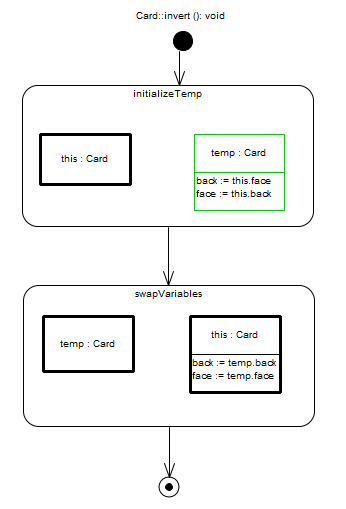
\includegraphics[width=0.7\textwidth]{ea_invertComplete}
  \caption{Swap back and face of the card}  
  \label{fig:sdm_invertComplete}
\end{center}
\end{figure}

\vspace{0.5cm}

\item[$\blacktriangleright$] Believe or not, that's it! Check out how this method was implemented in the textual syntax by reviewing
Fig.~\ref{fig:invertPatterns} on the next page.

\fancyfoot[R]{ $\triangleright$ \hyperlink{invert close}{Next}} 

\end{itemize}
